\documentclass[a4paper,12pt]{article}
\usepackage{amsmath}
\usepackage{amssymb}
\usepackage[polish]{babel}
\usepackage{polski}
\usepackage[utf8]{inputenc}
\usepackage{indentfirst}
\usepackage{geometry}
\usepackage{array}
\usepackage[pdftex]{color,graphicx}
\usepackage{subfigure}
\usepackage{afterpage}
\usepackage{setspace}
\usepackage{color}
\usepackage{wrapfig}
\usepackage{listings}
\usepackage{datetime}

\renewcommand{\onehalfspacing}{\setstretch{1.6}}

\geometry{tmargin=2.5cm,bmargin=2.5cm,lmargin=2.5cm,rmargin=2.5cm}
\setlength{\parindent}{1cm}
\setlength{\parskip}{0mm}

\newenvironment{lista}{
\begin{itemize}
  \setlength{\itemsep}{1pt}
  \setlength{\parskip}{0pt}
  \setlength{\parsep}{0pt}
}{\end{itemize}}

\newcommand{\linia}{\rule{\linewidth}{0.4mm}}

\definecolor{lbcolor}{rgb}{0.95,0.95,0.95}
\lstset{
    backgroundcolor=\color{lbcolor},
    tabsize=4,
  language=C++,
  captionpos=b,
  tabsize=3,
  frame=lines,
  numbers=left,
  numberstyle=\tiny,
  numbersep=5pt,
  breaklines=true,
  showstringspaces=false,
  basicstyle=\footnotesize,
  identifierstyle=\color{magenta},
  keywordstyle=\color[rgb]{0,0,1},
  commentstyle=\color{Darkgreen},
  stringstyle=\color{red}
  }

\begin{document}

\noindent
\begin{tabular}{|c|p{11cm}|c|} \hline 
Grupa 6 & Dariusz Szczupak, Kamil Wanat & \ddmmyyyydate\today \tabularnewline
\hline 
\end{tabular}


\section*{Zadanie 2 - Rozmycie Gaussa w MPI}

Celem zadania jest program oparty na algorytmie Gaussa mający na celu rozmycie danego zdjęcia. Zadanie wykonane z wykorzstaniem środowiska CUDA. "Gauss 2" - to użyta wersja filtru danego w dołączonym do treści zadania linku. Maska w danym filtrze wygląda następująco:

\begin{lstlisting}
int mask[5][5] = {{1,1,2,1,1}, {1,2,4,2,1}, {2,4,8,4,2}, {1,2,4,2,1}, {1,1,2,1,1}
};
\end{lstlisting}

Do obliczenia wartości z których składa się każdy piksel(Red, Green, Blue), potrzebne są punkty otaczające go. Każdy taki piksel ma jakąś wage, która z kolei zapisana jest w masce filtra. Liczymy sume ważoną kolejnych pixeli i jego sąsiadów, kolejnie dzielimy taką sumę przez sumę całej maski. Filtrowanie obrazu następuje oddzielnie dla każdej wartości z której składa się pixel. W metodzie filtrowania Gaussa znaczenie wartości pixela jest największe w punkcie, który jest liczony i zmniejsza się wraz z oddalaniem się od niego. Poniżej fragment kodu odpowiedzialny za wykonanie obliczeń dla składowych R, G, B:

\begin{lstlisting}
for (row = startForBlock; row < (startForBlock + blockSize); row++) {
        if (row >= rowsNumber) {
            break;
        }
        for (column = startForThread; column < (startForThread + threadSize); column++) {
            if (column >= columnsNumber) {
                break;
            }
            red = 0;
            green = 0;
            blue = 0;
            for (x = 0; x < 5; x++)
                for (y = 0; y < 5; y++) {
                    red += R[(row + x) * columnsNumber + column + y] * mask[x][y];
                    green += G[(row + x) * columnsNumber + column + y] * mask[x][y];
                    blue += B[(row + x) * columnsNumber + column + y] * mask[x][y];
                }
            resultRed[row * columnsNumber + column] = red / SumMask;
            resultGreen[row * columnsNumber + column] = green / SumMask;
            resultBlue[row * columnsNumber + column] = blue / SumMask;   
        }
    }      
\end{lstlisting}

Jest to fragment z funkcji globalnej (nazywanej kernelami). Funkcja globalna gaussianBlur jest wywoływana z poziomu hosta, ale wykonywana na urzadzeniu. Obrazek dzielony jest na paski według ilosci bloków. Paski te dzielone sa z kolei na małe skrawki w zaleznosci od ilosci watków. Ponizej przedstawiono wykres zaleznosci czasu od ilosci uzytych watków oraz wykres przyspieszenia:

\begin{figure}[!hbp]
	\centering
  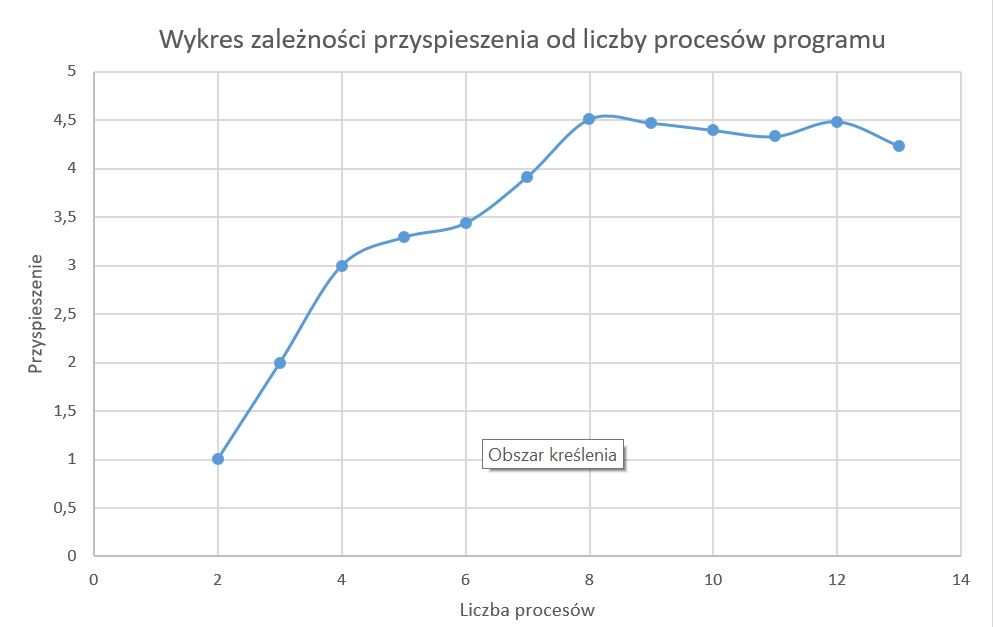
\includegraphics[width=0.7\textwidth]{wykres1.png}
  \caption{Wykres przyspieszenia}
\end{figure}


\begin{wrapfigure}{r}{0.5\textwidth}
  \vspace{-20pt}
  \begin{center}
  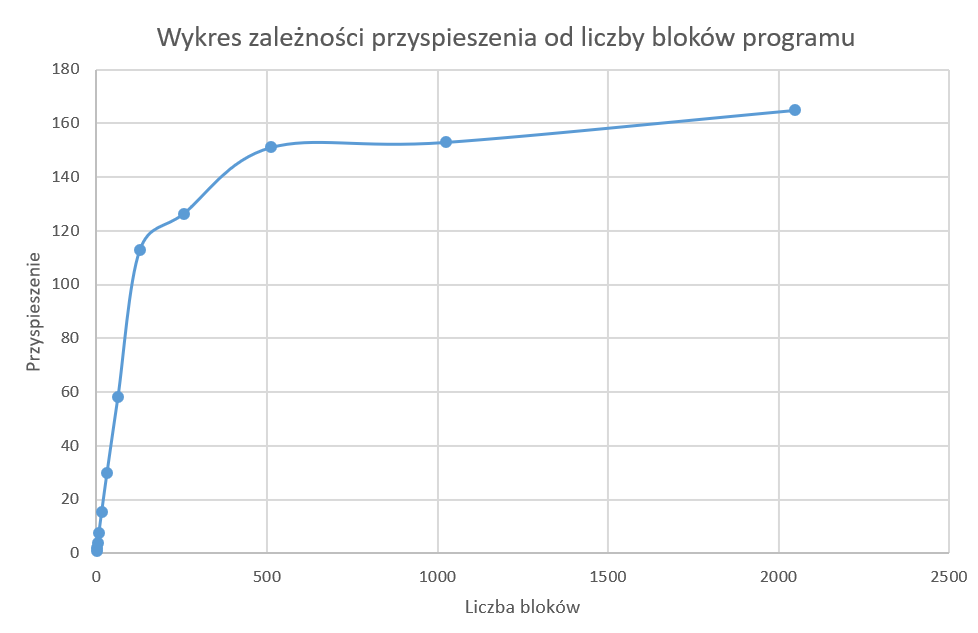
\includegraphics[width=0.45\textwidth]{wykres.png}
  \end{center}
  \vspace{-20pt}
  \caption{Wykres zależności czasu od liczby wątków}
  \vspace{-10pt}
\end{wrapfigure}

Z powyższych wykresów można wywnioskować że czas obliczeń spada gwałtownie miedzy 2 a 3 procesem po czym następuje stabilizacja.

Dane przeprowadzanych testów:
\begin{lista}
 \item Wzieto pod uwage srednia z 10 pomiarów czasów wykonania programu dla liczby
watków z przedziału od 1 do 1024. Program był uruchamiany dla obrazka ściągniętego z przestworzy internetów w rozdzielczośći 1920x1200px.
 \item Do mierzenia czasu wykorzystanoeventy z cudaEventElapsedTime.
 \item Do wczytania obrazu wykorzystano bibliotekę OpenCV .
 \item Testy zostały wykonane na serwerze cuda.iti.pk.edu.pl . 
\end{lista}
 
Zapoznaliśmy się z algorytmami i sposobami przetwarzania na karcie graficznej w
srodowisku CUDA. Zadanie udało się wykonać w całości. Dzieki zastosowaniu technologii CUDA mozna w sposób znaczacy przyspieszyc czas obliczen algorytmu rozmycia Gaussa. Najlepsze wyniki osiągnięto dla ilości wątków zbliżonej do ilości rdzeni procesora na serwerze CUDA. 


\end{document}